\documentclass{llncs}
\usepackage[portuguese]{babel}
\usepackage{times}
%\usepackage[utf8]{inputenc}
\usepackage[T1]{fontenc}


% Comentar para not MAC Users
\usepackage[applemac]{inputenc}

\usepackage{a4}
\usepackage[margin=3cm,nohead]{geometry}
\usepackage{epstopdf}
\usepackage{graphicx}
\usepackage{fancyvrb}
\usepackage{amsmath}
%\renewcommand{\baselinestretch}{1.5}

\begin{document}
\mainmatter
\title{Relat�rio do Trabalho Pr�tico de\\Programa��o Orientada a Objetos}

\titlerunning{Relat�rio do Trabalho TP de POO}

\author{ {El�sio Freitas Fernandes \{$55617$\}}  \and {Daniel Gon�alves Martins \{$73175$\}} \and {Nuno Jos� Ribeiro da Silva \{$78879$\}}}

\authorrunning{El�sio Fernandes \{$55617$\} \and Daniel Martins \{$73175$\} \and Nuno Silva {$78879$\} } }

\institute{
Universidade do Minho, Departamento de Informatica, 4710-057 Braga, Portugal\\
e-mail: \{a$55617$, a$73175$, a$78879$\}@uminho.pt
}

\date{}
\bibliographystyle{splncs}

\maketitle
\begin{abstract}
Serve o presente como relat�rio do projeto elaborado no �mbito da unidade curricular de Programa��o Orientada a Objetos. Projeto esse no qual se previa a elabora��o de um programa para a empresa UMeR, o qual fosse capaz de garantir a presta��o continua do seu servi�o. Os requisitos de tal programa incluem a cria��o e manuten��o da base de dados que inclui os dados dos clientes, bem como as informa��es dos seus colaboradores e das suas viaturas, utilizadas para a presta��o do servi�o em quest�o. Mais ainda, est� inclu�da a cria��o de uma interface de intera��o com os utilizadores com v�rias op��es, como: cria��o de conta; posterior acesso e atualiza��o dos dados da conta; consulta de hist�rico de servi�os requeridos/prestados.
\end{abstract}

\section{Introdu��o}

%N�o esquecer de referenciar apropriadamente...
 The present study proposes a novel and simple strategy to defined high-level unified QoS metrics for Internet services resorting to fuzzy logic principles \cite{Zadeh65}. 
 Attending to the specificity of the problem, which combines the difficulty of handling multiple low-level QoS parameters with the blur boundaries of user perceived QoS, the use of fuzzy logic to achieve a unique per service QoS metric brings a clear advantage and simplicity to the solution.
Fuzzy logic has two different meanings~\cite{Nguyen99}. ...

\section{One more section}

\subsection{One subsection}
abdc...
\subsection{One more...}

%UNCOMMENT se necess�rio
%De acordo com o ilustrado na Figura~\ref{fig:controller}
%% Exemplo para inser��o de uma figura
\begin{figure}
\begin{center}
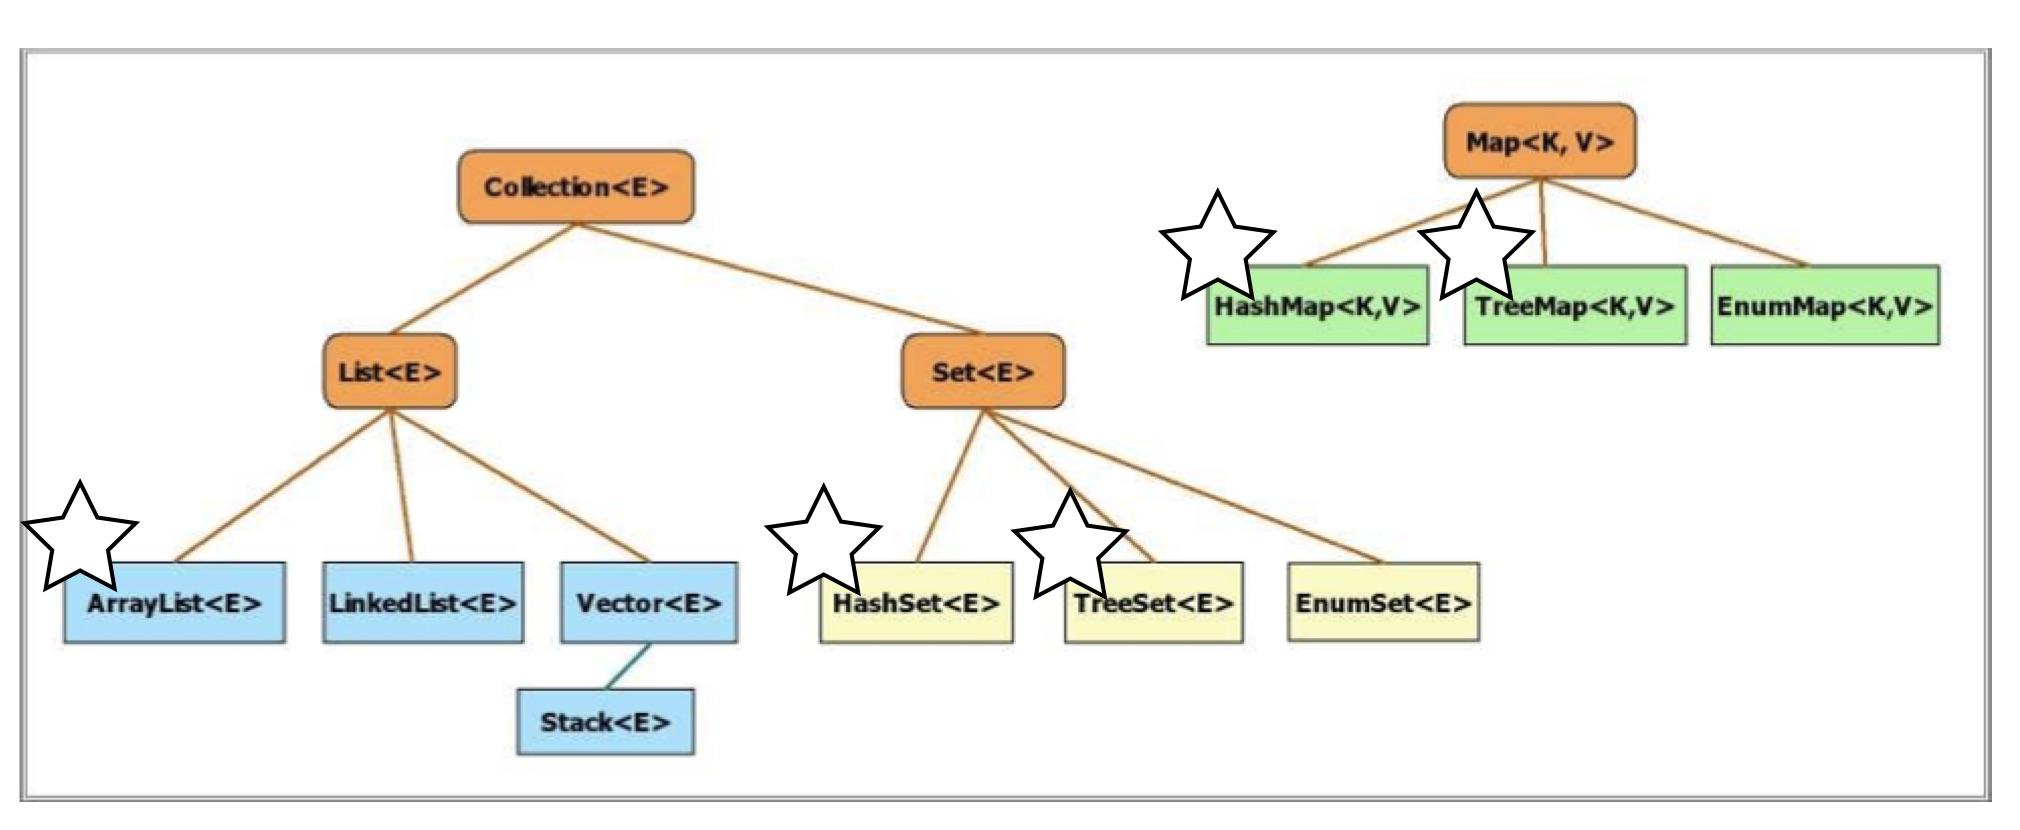
\includegraphics[scale=0.1]{collections.jpg} 
\end{center}
\caption{\label{fig:controller}Architecture of the unified QoS metric fuzzy controller.}
\end{figure} 

According to Table~\ref{tab:TabelaExemplo}...

% Exemplo de uma tabela com duas colunas
\begin{figure}
\centering
\begin{tabular}{|c|c|}\hline
(a) Delay and jiiter & (b) Delay and loss \\ \hline

(c) Delay and throughput & (d) Jitter and loss \\ \hline

(e) Jitter and throughput & (f) Loss and throughput \\ \hline
\end{tabular}
\caption{\label{tab:TabelaExemplo}Tabela exemplo.}
\end{figure}

%\section{Simulation Scenario}

\section{Conclusions}
Neste trabalho...

%UNCOMMENT para a bibliografia 
%% ficheirodebibliografia.bib
%\bibliography{ficheirodebibliografia}

%ou inserir directamente os v�rios \bibitem 
\begin{thebibliography}{1}
\bibitem{Zadeh65}
Zadeh, L.:
\newblock {Fuzzy sets} (1965)

\bibitem{Nguyen99}
Nguyen, H., Walker, E.:
\newblock {First course in fuzzy logic}.
\newblock {Boca Raton: Chapman and Hall/CRC Press} (1999)
\end{thebibliography}

\end{document}